\documentclass[tikz,border=10pt]{standalone}
\usepackage{tikz,amsmath}
\usetikzlibrary{arrows.meta, positioning, calc, decorations.pathmorphing, shadows.blur}

\begin{document}
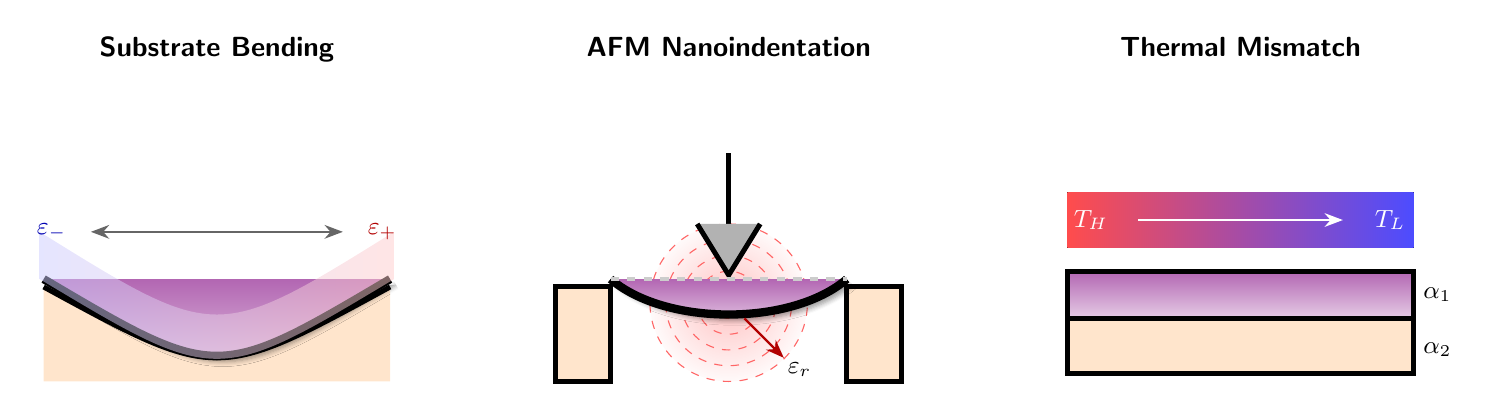
\begin{tikzpicture}[
    >=Stealth,
    font=\sffamily,
    symbol/.style={font=\sffamily\small},
    arrow/.style={->, thick},
    thickline/.style={line width=1.8pt, black},
    layer/.style={line width=3pt, draw=black, top color=violet!60, bottom color=violet!20, blur shadow={shadow blur steps=5}},
    gradientbar/.style={left color=red!70, right color=blue!70},
    title/.style={font=\bfseries\sffamily, align=center, anchor=north},
    label/.style={font=\sffamily\small}
]

% Title Y position
\def\titleY{3.2}

% ===== Panel 1: Substrate Bending =====
\begin{scope}[xshift=-6.5cm]
    \node[title] at (0,\titleY) {Substrate Bending};

    % Substrate
    \fill[orange!20] (-2.2,-0.1) .. controls (0,-1.3) .. (2.2,-0.1) -- (2.2,-1.3) -- (-2.2,-1.3) -- cycle;
    \draw[thickline] (-2.2,-0.1) .. controls (0,-1.3) .. (2.2,-0.1);

    % TMD layer
    \draw[layer] (-2.2,0) .. controls (0,-1.3) .. (2.2,0);

    % Gradient strain
    \shade[left color=blue!20, right color=red!20, opacity=0.5]
        (-2.25,0.0) .. controls (0,-1.35) .. (2.25,0.0) -- (2.25,0.6) .. controls (0,-0.8) .. (-2.25,0.6) -- cycle;

    % Strain arrows
    \draw[<->, thick, gray!80!black] (-1.6,0.6) -- (1.6,0.6);
    \node[label, red!70!black] at (2.1,0.6) {$\varepsilon_+$};
    \node[label, blue!70!black] at (-2.1,0.6) {$\varepsilon_-$};
\end{scope}

% ===== Panel 2: AFM Nanoindentation =====
\begin{scope}
    \node[title] at (0,\titleY) {AFM Nanoindentation};

    % Substrate supports
    \fill[orange!20] (-2.2,-1.3) rectangle (-1.5, -0.1);
    \fill[orange!20] (1.5,-1.3) rectangle (2.2, -0.1);
    \draw[thickline] (-2.2,-1.3) rectangle (-1.5, -0.1);
    \draw[thickline] (1.5,-1.3) rectangle (2.2, -0.1);

    % Indentation field
    \shade[inner color=red!60, outer color=red!5, opacity=0.4] (0,-0.3) circle (1);
    \foreach \r in {0.2,0.4,...,1.0} {
        \draw[red!60, dashed] (0,-0.3) circle (\r);
    }

    % AFM tip
    \draw[thickline] (0,1.6) -- (0,0.5);
    \fill[gray!60] (-0.4,0.7) -- (0,0.05) -- (0.4,0.7) -- cycle;
    \draw[thickline] (-0.4,0.7) -- (0,0.05) -- (0.4,0.7);

    % Membrane deformation
    \draw[layer] (-1.5,0) .. controls (-0.8,-0.6) and (0.8,-0.6) .. (1.5,0);
    \draw[black!20, line width=1.5pt, dashed] (-1.5,0) -- (1.5,0);

    % Strain arrow
    \draw[arrow, red!70!black] (0.2,-0.5) -- (0.7,-1);
    \node[label] at (0.9,-1.15) {$\varepsilon_r$};
\end{scope}

% ===== Panel 3: Thermal Mismatch =====
\begin{scope}[xshift=6.5cm]
    \node[title] at (0,\titleY) {Thermal Mismatch};

    % Gradient temperature bar
    \fill[gradientbar] (-2.2,1.1) rectangle (2.2,0.4);
    \draw[->, white, thick] (-1.3,0.75) -- (1.3,0.75);
    \node[label, white] at (-1.9,0.75) {$T_H$};
    \node[label, white] at (1.9,0.75) {$T_L$};

    % Substrate
    \fill[orange!20] (-2.2,-0.5) rectangle (2.2,-1.2);
    \draw[thickline] (-2.2,-0.5) rectangle (2.2,-1.2);

    % TMD Layer
    \fill[top color=violet!60, bottom color=violet!20] (-2.2,0.1) rectangle (2.2,-0.5);
    \draw[thickline] (-2.2,0.1) rectangle (2.2,-0.5);

    % Expansion coefficients
    \node[label] at (2.5,-0.2) {$\alpha_1$};
    \node[label] at (2.5,-0.9) {$\alpha_2$};
\end{scope}

\end{tikzpicture}
\end{document}
